\section{Automatically Diversifying Tie-breaking using OpenTrees}

Although the above technique provides an interesting worst case guarantee, the coverage results in \reftbl{single-coverage} are not so overwhelmingly good compared to single LIFO strategy. The next step we have is whether there is a dominating strategy which outperforms all such vaiants.

In the previous section we observed that the search in a plateau is \emph{knowledge free} in terms of $f$ or $h$ value. The \sota knowledge free search algorithm widely used in the Robotics community is Rapidily-exploring Random Tree(RRT), which quickly expands a space-filling tree in a coninuous space using a state sampling.  RRT has a tree whose node is a state and the edge is a path between those states.
RRT uniformly samples a state in the state space, find its nearest neighboring node in the current tree, then extend the node by adding a new edge and node which slightly approach to the sampled state. The path is computed by a local planner.
This allows the motion planner to search the most unexplored volonoi region of the space and stochastically achieves an asymptotically complete space-filling tree.
In contrast, a trivial strategy to expand the tree by picking a node randomly out of the nodes in a tree does not achieve the same space-filling behavior. This is because by this strategy, the node near the root is selected in the same probability as the node that are far from the root.

\begin{figure}[htbp]
 \centering
 \relsize{-2}
 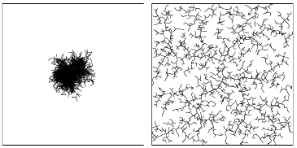
\includegraphics{img/trivial-vs-rrt.png}
 \caption{Trivial vs Rapidly exploring Random Tree with 2000 vertices. Picture is taken from \cite{lavalle2001randomized}.}
 \label{rrt}
\end{figure}

The difficulty in adapting RRT to a discrete state space search is how to sample the state uniformly, as well as $O(n^2)$ distance computations required in each step of adding a new node to the tree \cite{alcazar2011adapting}. The previous approaches tacked the first issue by sampling states which are reachable from the initial state \cite{alcazar2011adapting}. The second issue is far more problematic: In particular, let alone the $O(n^2)$ computation on each node expansion is very expensive since actually this $n$ is exponentially large, each distance computation is same as an individual planning problem, which is computationally intractable. Previous approaches tried to overcome this issue by relaxing the plan distance to distance estimate which can be computed in polynomial time, such as \ff heuristics. 
However, \ff heuristics are also decently computationally heavy compared to the euclidean distance used in motion plannning community.

\subsection{OpenTrees}

Now we introduce OpenTrees, which replaces the traditional open list and tiebreaking approaches and achieves the similar behavior as RRT.
It does not require the expensive distance computation, nor imply the plan distance between the states.
Notably, the use of OpenTrees does not violate admissibility. Both previous approaches in adapting RRT to planning are aimed at satisficing planning setting because they use RRT as the overall framework, while \sota approaches like $A^*$ only as the local planner. In contrast, we use the similar approach only in searching the plateau \emph{within} the same $f$ value. Moreover, search on plateaus is \emph{essentially knowledge free} and naturally suitable for RRT-like algorithms.

OpenTrees is a priority queue whose elements are the trees instead of arrays. Each nodes of the tree corresponds to a search state and each edge corresponds to an action.
The root node is the initial state and the the open states are stored in the leaf nodes.
The non-leaf nodes, including the root, are called a \emph{helper} nodes.

When an insertion of a new node happens, it first selects a tree with the same $f$ as the node, and then tries to insert the path from the initial state to the node into the tree. If a node is removed from the OpenTree, then unnecessary helper nodes should also be removed. The next state to expand are selected as follows: Starting from the root node of the current minimum $f$ value, select one branch at random at each step, until the node is a leaf node. Finally, return the leaf node.

\begin{figure}[htbp]
 \centering
 \relsize{-2}
 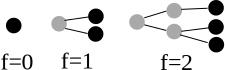
\includegraphics{img/trees.png}
 \caption{Figure depicting OpenTrees.}
 \label{trees}
\end{figure}

\subsection{Theoretical Analysis of OpenTrees}

An OpenTrees stochastically returns a state in a branch of the search tree with the least number of leaf nodes. Consider two nodes $n_1,n_2$ in \refig{probability}. These are directly generated from a parent node $n_p$ by different actions $a_1,a_2$. Their paths from the initial state only differs in this single step, in other words they share the very long path prefix. The probability of selecting the branch of $n_p$ is evenly shared by $n_1,n_2$ -- it becomes the half of selecting $n_p$. Thus, a path which have a longer prefix shared with another path has a smaller probability to be opened first (although they should be opened eventually when the current OpenTrees is exhausted), and OpenTrees returns the most surprizing node in terms of path difference.
This results in maximising the surprisal of the path that leads to the returned node.
% This results in returning a state which has the largest ``surprise'' in terms of the pathes that leads to the open nodes.

% \begin{figure}[htbp]
%  \centering
%  \relsize{-2}
%  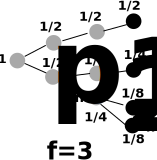
\includegraphics{img/open-tree-probability.png}
%  \caption{The probability of each leaf node to be opened, along with the probability of the helper % nodes to be visited. The nodes in a branch already heavily expanded are selected in a smaller % possibility, and the nodes in a narrower branch gets the higher possibility. It thus manages the % diversity of the search.}
%  \label{probability}
% \end{figure}

The novelty of this algrithm compared to the previous RRT-A* combinations is that we adopted the edit distance of the paths instead of state distance e.g. plan distance or relaxed plan distance.
Comppared to the plan distance, path distance is very easy to compute. Also, OpenTree implicitly balances the diversity of the search avoiding the costly $O(n^2)$ Nearest Neighbor Search.

\subsection{Experimental Results}
\label{sec-3}

We conducted experiments on 3 tractable heuristic functions, blind, $h^{\mbox{max}}$ and Landmark Cut heuristics (LMcut) \cite{Helmert2009}, as well as the intractable heuristics such as almost perfect heuristics with $c=3$ and the perfect heuristics.

In evaluating our approach on tractable heuristic functions, we applied a standard competition settings of 30min.\ time limit and 2GB memory limit.

In the experiments simulating almost perfect heuristics and perfect
heuristics, time limit is not applied and the heuristic values are computed by searching
from the node to the goal using optimal planning with LMcut. Thus, the
problem instances used in these settings are limited to the small instances.

The coverage results in \reftbl{tbl:main} show that OpenTrees significantly improves upon \astar across the tractable functions, and also across the intractable functions. We also show that the number of expansions in OpenTrees is significantly smaller than that of \astar. Note that the number of expansion when the heuristic estimate is larger than zero is the same between these two algorithms.

%The implications here is that the diversity information is orthogonal to the information %obtained from the distance estimation. In intractable heuristics, we can assume nearly all %information from the domain, current state and the goal state is obtained because we cannot %improve upon perfect heuristics. The only remaining unexploited information is left in the %relationship between the search nodes.
{ \setlength{\tabcolsep}{0.1em}
\begin{table}[htbp]
\centering \relsize{-1}
\begin{tabular}{|l|ll|ll||ll|}
\hline
 & blind &  & LMcut &  & Almost & Perfect  \\
 &  &  &  &  & $c=3$ &   \\
Domains & \astar & OT & \astar & OT & \astar & OT  \\
\hline
Gripper(20) & 9 & 10 & 12 & \textbf{13} &  &   \\
Depot(20) & 11 & 11 & 15 & \textbf{20} &  &   \\
Airport(30) & \ldots{} &  &  &  &  &  \\
TPP &  &  &  &  &  &   \\
CyberSec &  &  &  &  &  & \\
Sokoban &  &  &  &  &  &  \\
\ldots{} &  &  &  &  &  &  \\
\ldots{} &  &  &  &  &  &  \\
\ldots{} &  &  &  &  &  &  \\
\ldots{} &  &  &  &  &  &  \\
\ldots{} &  &  &  &  &  &  \\
expected & wi & dth & and & hei & ght & \\
\ldots{} &  &  &  &  &  & \\
\ldots{} &  &  &  &  &  & \\
\ldots{} &  &  &  &  &  & \\
\ldots{} &  &  &  &  &  & \\
\ldots{} &  &  &  &  &  & \\
\ldots{} &  &  &  &  &  & \\
\ldots{} &  &  &  &  &  & \\
Zenotravel &  &  &  &  &  & \\
\hline
Total & 800 & \textbf{900} &  &  &  & \\
\hline
\end{tabular}
\caption{The coverage results of \astar and $^*A^*$ with 30 min experiments on 2 GB machine. Best results across the tractable heuristics are indicated in \textbf{bold}.}
\label{tbl:main}
\end{table}

}

In \refig{diversity-transition}, we plotted the transition of diversity in the plateau as the expansion continues. The $y$-axis, the diversity across the plateau, was computed according to the formula $D(S_o)=abc/def$ where $S_o$ is the set of states with the best f-value in the open list. The $x$-axis in the figure shows the ratio of the size of $S_o$ to the size of $S_c$, the set of states in the closed list with best f-value, indicating the search progress.

It shows that the diversity in the open list remains high in OpenTrees, while it quickly decreases in \astar. It indicates that the expansion is done evenly on various kinds of nodes, rather than in a biased manner that the expansion is focused on a particular set of nodes.
% \todo{of course, the real figure should not be an ASCII art!}

\begin{figure}[htbp]
\begin{verbatim}
LMcut          Almost Perfect       

D(S)             D(S)                             
|                |             
||\___OpenTrees  ||\___OpenTrees
|\    \____      |\    \____   
| \        \__   | \        \__
|  ~\ A*+FIFO    |  ~\ A*+FIFO 
|    ~-_______   |    ~-_______
+------------->  +------------->
      #(S_c)/#(S_o)     #(S_c)/#(S_o)
\end{verbatim}
\caption{Transition of the diversity in the unexpanded best-f nodes in the open list.}
\label{diversity-transition}
\end{figure}
